% Options for packages loaded elsewhere
\PassOptionsToPackage{unicode}{hyperref}
\PassOptionsToPackage{hyphens}{url}
%
\documentclass[
]{article}
\usepackage{amsmath,amssymb}
\usepackage{lmodern}
\usepackage{iftex}
\ifPDFTeX
  \usepackage[T1]{fontenc}
  \usepackage[utf8]{inputenc}
  \usepackage{textcomp} % provide euro and other symbols
\else % if luatex or xetex
  \usepackage{unicode-math}
  \defaultfontfeatures{Scale=MatchLowercase}
  \defaultfontfeatures[\rmfamily]{Ligatures=TeX,Scale=1}
\fi
% Use upquote if available, for straight quotes in verbatim environments
\IfFileExists{upquote.sty}{\usepackage{upquote}}{}
\IfFileExists{microtype.sty}{% use microtype if available
  \usepackage[]{microtype}
  \UseMicrotypeSet[protrusion]{basicmath} % disable protrusion for tt fonts
}{}
\makeatletter
\@ifundefined{KOMAClassName}{% if non-KOMA class
  \IfFileExists{parskip.sty}{%
    \usepackage{parskip}
  }{% else
    \setlength{\parindent}{0pt}
    \setlength{\parskip}{6pt plus 2pt minus 1pt}}
}{% if KOMA class
  \KOMAoptions{parskip=half}}
\makeatother
\usepackage{xcolor}
\usepackage[margin=1in]{geometry}
\usepackage{graphicx}
\makeatletter
\def\maxwidth{\ifdim\Gin@nat@width>\linewidth\linewidth\else\Gin@nat@width\fi}
\def\maxheight{\ifdim\Gin@nat@height>\textheight\textheight\else\Gin@nat@height\fi}
\makeatother
% Scale images if necessary, so that they will not overflow the page
% margins by default, and it is still possible to overwrite the defaults
% using explicit options in \includegraphics[width, height, ...]{}
\setkeys{Gin}{width=\maxwidth,height=\maxheight,keepaspectratio}
% Set default figure placement to htbp
\makeatletter
\def\fps@figure{htbp}
\makeatother
\setlength{\emergencystretch}{3em} % prevent overfull lines
\providecommand{\tightlist}{%
  \setlength{\itemsep}{0pt}\setlength{\parskip}{0pt}}
\setcounter{secnumdepth}{-\maxdimen} % remove section numbering
\usepackage{booktabs}
\usepackage{longtable}
\usepackage{array}
\usepackage{multirow}
\usepackage{wrapfig}
\usepackage{float}
\usepackage{colortbl}
\usepackage{pdflscape}
\usepackage{tabu}
\usepackage{threeparttable}
\usepackage{threeparttablex}
\usepackage[normalem]{ulem}
\usepackage{makecell}
\usepackage{xcolor}
\ifLuaTeX
  \usepackage{selnolig}  % disable illegal ligatures
\fi
\IfFileExists{bookmark.sty}{\usepackage{bookmark}}{\usepackage{hyperref}}
\IfFileExists{xurl.sty}{\usepackage{xurl}}{} % add URL line breaks if available
\urlstyle{same} % disable monospaced font for URLs
\hypersetup{
  pdftitle={Statin Simulation Report},
  pdfauthor={Haodong Li},
  hidelinks,
  pdfcreator={LaTeX via pandoc}}

\title{Statin Simulation Report}
\author{Haodong Li}
\date{2022-10-03}

\begin{document}
\maketitle

\hypertarget{simulation}{%
\subsection{Simulation}\label{simulation}}

\underline{DGD:} \begin{eqnarray*}
W_{1} &\sim& Unif(-1, 1)\\[1pt]
W_{2} &\sim& Unif(-1, 1)\\[1pt]
A &\sim& Bernoulli(p) \mbox{~~where~~} p = \mbox{expit}(0.1*W_1*W_2-0.4*W_1) \\[1pt]
\tau &=& W_1^2*(W_1+7/5) + (5*W_2/3)^2\\[1pt]
\mu_{Y} &=& A*\tau + W_1*W_2 + 2*W_2^2 - W_1 \\[1pt]
Y &\sim& N(\mu_{Y}, 1)
\end{eqnarray*}

\underline{Initial estimating models for Q and g:}

\begin{enumerate}
\def\labelenumi{\arabic{enumi})}
\item
  GAM: General Additive Models (Correctly specified based on true DGD of
  Q and g)
\item
  Earth: Multivariate Adaptive Regression Splines
\end{enumerate}

Note this is not SL, just individual algorithms. For estimations of
other terms (\(\tau,\tau_s,\gamma_s\)), all use Earth.

\underline{CATE estimation}

\begin{enumerate}
\def\labelenumi{\arabic{enumi})}
\item
  DR-learner: regress pseudo outcome estimates \(\varphi_n^0\) on \(W\).
\item
  T-learner: just use \(\bar{Q}_n^0(1,W)\) - \(\bar{Q}_n^0(0,W)\)
\end{enumerate}

\underline{Truncation:}

For TMLE, \(\bar{Q}_n^{_{(0)}}\) \(\in\) \([0.001, 0.999]\), \(g_n\)
\(\in\) \([0.025, 0.975]\).

For EE, \(g_n\) \(\in\) \([0.025, 0.975]\)

\begin{table}

\caption{\label{tab:unnamed-chunk-5}Configuration of simulations}
\centering
\fontsize{10}{12}\selectfont
\begin{tabular}[t]{llll}
\toprule
Table\_ID & Model\_Q\_g & CATE\_learner & CV\\
\midrule
Table 2 & GAM & DR-learner & No\\
Table 3 & GAM & T-learner & No\\
Table 4 & Earth & DR-learner & No\\
Table 5 & Earth & T-learner & No\\
\addlinespace
Table 6 & GAM & DR-learner & Yes\\
Table 7 & GAM & T-learner & Yes\\
Table 8 & Earth & DR-learner & Yes\\
Table 9 & Earth & T-learner & Yes\\
\bottomrule
\end{tabular}
\end{table}

\begin{table}

\caption{\label{tab:unnamed-chunk-6}Performance of TMLE and EE for Theta (Correct Q and g, DR-learner, no CV)}
\centering
\resizebox{\linewidth}{!}{
\begin{tabular}[t]{rlrrrrrrr}
\toprule
n & Method & True\_Theta & Variance & Bias & MSE & Coverage & Coverage\_or & CI\_width\\
\midrule
 & TMLE & 0.686 & 0.0265 & 0.0302 & 0.0275 & 0.938 & 0.948 & 0.6386\\

\multirow{-2}{*}{\raggedleft\arraybackslash 500} & EE & 0.686 & 0.0414 & 0.0758 & 0.0472 & 0.914 & 0.928 & 0.7010\\
\cmidrule{1-9}
 & TMLE & 0.686 & 0.0124 & 0.0100 & 0.0125 & 0.950 & 0.954 & 0.4369\\

\multirow{-2}{*}{\raggedleft\arraybackslash 1000} & EE & 0.686 & 0.0165 & 0.0430 & 0.0183 & 0.930 & 0.942 & 0.4652\\
\cmidrule{1-9}
 & TMLE & 0.686 & 0.0056 & 0.0070 & 0.0057 & 0.958 & 0.956 & 0.3062\\

\multirow{-2}{*}{\raggedleft\arraybackslash 2000} & EE & 0.686 & 0.0061 & 0.0272 & 0.0068 & 0.942 & 0.928 & 0.3145\\
\cmidrule{1-9}
 & TMLE & 0.686 & 0.0040 & 0.0112 & 0.0041 & 0.946 & 0.940 & 0.2504\\

\multirow{-2}{*}{\raggedleft\arraybackslash 3000} & EE & 0.686 & 0.0041 & 0.0215 & 0.0046 & 0.942 & 0.938 & 0.2538\\
\cmidrule{1-9}
 & TMLE & 0.686 & 0.0029 & 0.0054 & 0.0030 & 0.952 & 0.952 & 0.2152\\

\multirow{-2}{*}{\raggedleft\arraybackslash 4000} & EE & 0.686 & 0.0031 & 0.0106 & 0.0032 & 0.954 & 0.952 & 0.2169\\
\cmidrule{1-9}
 & TMLE & 0.686 & 0.0023 & 0.0038 & 0.0023 & 0.956 & 0.952 & 0.1925\\

\multirow{-2}{*}{\raggedleft\arraybackslash 5000} & EE & 0.686 & 0.0023 & 0.0046 & 0.0023 & 0.958 & 0.946 & 0.1931\\
\cmidrule{1-9}
 & TMLE & 0.686 & 0.0013 & 0.0060 & 0.0013 & 0.934 & 0.938 & 0.1364\\

\multirow{-2}{*}{\raggedleft\arraybackslash 10000} & EE & 0.686 & 0.0013 & 0.0000 & 0.0013 & 0.934 & 0.946 & 0.1360\\
\cmidrule{1-9}
 & TMLE & 0.686 & 0.0006 & 0.0079 & 0.0007 & 0.938 & 0.940 & 0.0966\\

\multirow{-2}{*}{\raggedleft\arraybackslash 20000} & EE & 0.686 & 0.0006 & -0.0017 & 0.0006 & 0.948 & 0.944 & 0.0960\\
\bottomrule
\end{tabular}}
\end{table}

\begin{table}

\caption{\label{tab:unnamed-chunk-7}Performance of TMLE and EE for Theta (Correct Q and g, T-learner, no CV)}
\centering
\resizebox{\linewidth}{!}{
\begin{tabular}[t]{rlrrrrrrr}
\toprule
n & Method & True\_Theta & Variance & Bias & MSE & Coverage & Coverage\_or & CI\_width\\
\midrule
 & TMLE & 0.686 & 0.0234 & 0.0276 & 0.0242 & 0.954 & 0.954 & 0.6279\\

\multirow{-2}{*}{\raggedleft\arraybackslash 500} & EE & 0.686 & 0.0238 & 0.0442 & 0.0257 & 0.944 & 0.946 & 0.6111\\
\cmidrule{1-9}
 & TMLE & 0.686 & 0.0113 & 0.0179 & 0.0116 & 0.954 & 0.936 & 0.4373\\

\multirow{-2}{*}{\raggedleft\arraybackslash 1000} & EE & 0.686 & 0.0112 & 0.0285 & 0.0120 & 0.950 & 0.934 & 0.4287\\
\cmidrule{1-9}
 & TMLE & 0.686 & 0.0061 & 0.0121 & 0.0062 & 0.952 & 0.932 & 0.3062\\

\multirow{-2}{*}{\raggedleft\arraybackslash 2000} & EE & 0.686 & 0.0061 & 0.0161 & 0.0064 & 0.940 & 0.932 & 0.3024\\
\cmidrule{1-9}
 & TMLE & 0.686 & 0.0039 & 0.0082 & 0.0040 & 0.944 & 0.948 & 0.2488\\

\multirow{-2}{*}{\raggedleft\arraybackslash 3000} & EE & 0.686 & 0.0039 & 0.0106 & 0.0040 & 0.944 & 0.952 & 0.2466\\
\cmidrule{1-9}
 & TMLE & 0.686 & 0.0026 & 0.0057 & 0.0027 & 0.964 & 0.952 & 0.2154\\

\multirow{-2}{*}{\raggedleft\arraybackslash 4000} & EE & 0.686 & 0.0026 & 0.0073 & 0.0027 & 0.964 & 0.944 & 0.2137\\
\cmidrule{1-9}
 & TMLE & 0.686 & 0.0024 & 0.0090 & 0.0025 & 0.956 & 0.950 & 0.1929\\

\multirow{-2}{*}{\raggedleft\arraybackslash 5000} & EE & 0.686 & 0.0024 & 0.0101 & 0.0025 & 0.946 & 0.944 & 0.1915\\
\cmidrule{1-9}
 & TMLE & 0.686 & 0.0012 & 0.0057 & 0.0012 & 0.952 & 0.944 & 0.1363\\

\multirow{-2}{*}{\raggedleft\arraybackslash 10000} & EE & 0.686 & 0.0012 & 0.0058 & 0.0012 & 0.954 & 0.942 & 0.1358\\
\cmidrule{1-9}
 & TMLE & 0.686 & 0.0005 & 0.0044 & 0.0006 & 0.960 & 0.952 & 0.0962\\

\multirow{-2}{*}{\raggedleft\arraybackslash 20000} & EE & 0.686 & 0.0005 & 0.0041 & 0.0006 & 0.958 & 0.952 & 0.0960\\
\bottomrule
\end{tabular}}
\end{table}

\begin{table}

\caption{\label{tab:unnamed-chunk-8}Performance of TMLE and EE for Theta (earth est Q and g, DR-learner, no CV)}
\centering
\resizebox{\linewidth}{!}{
\begin{tabular}[t]{rlrrrrrrr}
\toprule
n & Method & True\_Theta & Variance & Bias & MSE & Coverage & Coverage\_or & CI\_width\\
\midrule
 & TMLE & 0.686 & 0.0930 & 0.0069 & 0.0930 & 0.918 & 0.978 & 0.7526\\

\multirow{-2}{*}{\raggedleft\arraybackslash 500} & EE & 0.686 & 0.3765 & 0.1823 & 0.4097 & 0.920 & 0.968 & 1.1256\\
\cmidrule{1-9}
 & TMLE & 0.686 & 0.0274 & -0.0071 & 0.0275 & 0.932 & 0.980 & 0.4766\\

\multirow{-2}{*}{\raggedleft\arraybackslash 1000} & EE & 0.686 & 0.0467 & 0.0648 & 0.0509 & 0.932 & 0.972 & 0.5946\\
\cmidrule{1-9}
 & TMLE & 0.686 & 0.0077 & -0.0053 & 0.0077 & 0.944 & 0.964 & 0.3217\\

\multirow{-2}{*}{\raggedleft\arraybackslash 2000} & EE & 0.686 & 0.0245 & 0.0496 & 0.0269 & 0.952 & 0.964 & 0.4007\\
\cmidrule{1-9}
 & TMLE & 0.686 & 0.0053 & -0.0072 & 0.0053 & 0.920 & 0.960 & 0.2539\\

\multirow{-2}{*}{\raggedleft\arraybackslash 3000} & EE & 0.686 & 0.0071 & 0.0293 & 0.0080 & 0.926 & 0.954 & 0.2831\\
\cmidrule{1-9}
 & TMLE & 0.686 & 0.0032 & -0.0148 & 0.0035 & 0.934 & 0.950 & 0.2171\\

\multirow{-2}{*}{\raggedleft\arraybackslash 4000} & EE & 0.686 & 0.0056 & 0.0157 & 0.0059 & 0.952 & 0.976 & 0.2379\\
\cmidrule{1-9}
 & TMLE & 0.686 & 0.0027 & -0.0170 & 0.0029 & 0.930 & 0.944 & 0.1978\\

\multirow{-2}{*}{\raggedleft\arraybackslash 5000} & EE & 0.686 & 0.0033 & 0.0075 & 0.0033 & 0.958 & 0.964 & 0.2069\\
\cmidrule{1-9}
 & TMLE & 0.686 & 0.0014 & -0.0174 & 0.0017 & 0.884 & 0.922 & 0.1360\\

\multirow{-2}{*}{\raggedleft\arraybackslash 10000} & EE & 0.686 & 0.0013 & -0.0018 & 0.0013 & 0.926 & 0.944 & 0.1379\\
\cmidrule{1-9}
 & TMLE & 0.686 & 0.0006 & -0.0160 & 0.0009 & 0.876 & 0.896 & 0.0957\\

\multirow{-2}{*}{\raggedleft\arraybackslash 20000} & EE & 0.686 & 0.0006 & -0.0036 & 0.0006 & 0.942 & 0.950 & 0.0968\\
\bottomrule
\end{tabular}}
\end{table}

\begin{table}

\caption{\label{tab:unnamed-chunk-9}Performance of TMLE and EE for Theta (earth est Q and g, T-learner, no CV)}
\centering
\resizebox{\linewidth}{!}{
\begin{tabular}[t]{rlrrrrrrr}
\toprule
n & Method & True\_Theta & Variance & Bias & MSE & Coverage & Coverage\_or & CI\_width\\
\midrule
 & TMLE & 0.686 & 0.0239 & 0.0121 & 0.0240 & 0.958 & 0.962 & 0.6459\\

\multirow{-2}{*}{\raggedleft\arraybackslash 500} & EE & 0.686 & 0.0254 & -0.0018 & 0.0255 & 0.962 & 0.956 & 0.6530\\
\cmidrule{1-9}
 & TMLE & 0.686 & 0.0114 & 0.0093 & 0.0115 & 0.958 & 0.940 & 0.4492\\

\multirow{-2}{*}{\raggedleft\arraybackslash 1000} & EE & 0.686 & 0.0122 & -0.0005 & 0.0122 & 0.952 & 0.940 & 0.4557\\
\cmidrule{1-9}
 & TMLE & 0.686 & 0.0065 & 0.0002 & 0.0065 & 0.946 & 0.948 & 0.3133\\

\multirow{-2}{*}{\raggedleft\arraybackslash 2000} & EE & 0.686 & 0.0066 & -0.0051 & 0.0066 & 0.942 & 0.948 & 0.3171\\
\cmidrule{1-9}
 & TMLE & 0.686 & 0.0042 & -0.0053 & 0.0042 & 0.934 & 0.936 & 0.2500\\

\multirow{-2}{*}{\raggedleft\arraybackslash 3000} & EE & 0.686 & 0.0043 & -0.0088 & 0.0044 & 0.944 & 0.940 & 0.2529\\
\cmidrule{1-9}
 & TMLE & 0.686 & 0.0028 & -0.0087 & 0.0029 & 0.942 & 0.940 & 0.2165\\

\multirow{-2}{*}{\raggedleft\arraybackslash 4000} & EE & 0.686 & 0.0028 & -0.0107 & 0.0029 & 0.946 & 0.942 & 0.2186\\
\cmidrule{1-9}
 & TMLE & 0.686 & 0.0025 & -0.0060 & 0.0026 & 0.942 & 0.946 & 0.1924\\

\multirow{-2}{*}{\raggedleft\arraybackslash 5000} & EE & 0.686 & 0.0026 & -0.0082 & 0.0026 & 0.942 & 0.946 & 0.1946\\
\cmidrule{1-9}
 & TMLE & 0.686 & 0.0012 & -0.0099 & 0.0013 & 0.942 & 0.944 & 0.1355\\

\multirow{-2}{*}{\raggedleft\arraybackslash 10000} & EE & 0.686 & 0.0012 & -0.0108 & 0.0013 & 0.938 & 0.946 & 0.1372\\
\cmidrule{1-9}
 & TMLE & 0.686 & 0.0006 & -0.0119 & 0.0007 & 0.920 & 0.920 & 0.0955\\

\multirow{-2}{*}{\raggedleft\arraybackslash 20000} & EE & 0.686 & 0.0006 & -0.0125 & 0.0007 & 0.924 & 0.916 & 0.0966\\
\bottomrule
\end{tabular}}
\end{table}

\begin{table}

\caption{\label{tab:unnamed-chunk-10}Performance of TMLE and EE for Theta (Correct Q and g, DR-learner, CV)}
\centering
\resizebox{\linewidth}{!}{
\begin{tabular}[t]{rlrrrrrrr}
\toprule
n & Method & True\_Theta & Variance & Bias & MSE & Coverage & Coverage\_or & CI\_width\\
\midrule
 & TMLE & 0.686 & 0.0299 & 0.0302 & 0.0308 & 0.964 & 0.960 & 0.6897\\

\multirow{-2}{*}{\raggedleft\arraybackslash 500} & EE & 0.686 & 0.0868 & -0.1703 & 0.1158 & 0.852 & 0.962 & 0.8408\\
\cmidrule{1-9}
 & TMLE & 0.686 & 0.0129 & 0.0162 & 0.0132 & 0.960 & 0.950 & 0.4583\\

\multirow{-2}{*}{\raggedleft\arraybackslash 1000} & EE & 0.686 & 0.0168 & -0.0946 & 0.0257 & 0.870 & 0.894 & 0.4990\\
\cmidrule{1-9}
 & TMLE & 0.686 & 0.0058 & 0.0072 & 0.0059 & 0.960 & 0.954 & 0.3119\\

\multirow{-2}{*}{\raggedleft\arraybackslash 2000} & EE & 0.686 & 0.0068 & -0.0512 & 0.0094 & 0.902 & 0.914 & 0.3246\\
\cmidrule{1-9}
 & TMLE & 0.686 & 0.0041 & 0.0094 & 0.0041 & 0.948 & 0.944 & 0.2536\\

\multirow{-2}{*}{\raggedleft\arraybackslash 3000} & EE & 0.686 & 0.0045 & -0.0306 & 0.0054 & 0.908 & 0.930 & 0.2594\\
\cmidrule{1-9}
 & TMLE & 0.686 & 0.0030 & 0.0040 & 0.0030 & 0.964 & 0.956 & 0.2169\\

\multirow{-2}{*}{\raggedleft\arraybackslash 4000} & EE & 0.686 & 0.0032 & -0.0231 & 0.0038 & 0.918 & 0.932 & 0.2202\\
\cmidrule{1-9}
 & TMLE & 0.686 & 0.0023 & 0.0023 & 0.0023 & 0.958 & 0.954 & 0.1937\\

\multirow{-2}{*}{\raggedleft\arraybackslash 5000} & EE & 0.686 & 0.0024 & -0.0206 & 0.0028 & 0.922 & 0.922 & 0.1956\\
\cmidrule{1-9}
 & TMLE & 0.686 & 0.0013 & 0.0036 & 0.0013 & 0.930 & 0.946 & 0.1366\\

\multirow{-2}{*}{\raggedleft\arraybackslash 10000} & EE & 0.686 & 0.0013 & -0.0084 & 0.0014 & 0.918 & 0.936 & 0.1367\\
\cmidrule{1-9}
 & TMLE & 0.686 & 0.0006 & 0.0055 & 0.0006 & 0.936 & 0.936 & 0.0966\\

\multirow{-2}{*}{\raggedleft\arraybackslash 20000} & EE & 0.686 & 0.0006 & -0.0053 & 0.0006 & 0.942 & 0.946 & 0.0962\\
\bottomrule
\end{tabular}}
\end{table}

\begin{table}

\caption{\label{tab:unnamed-chunk-11}Performance of TMLE and EE for Theta (Correct Q and g, T-learner, CV)}
\centering
\resizebox{\linewidth}{!}{
\begin{tabular}[t]{rlrrrrrrr}
\toprule
n & Method & True\_Theta & Variance & Bias & MSE & Coverage & Coverage\_or & CI\_width\\
\midrule
 & TMLE & 0.686 & 0.0252 & -0.0295 & 0.0261 & 0.926 & 0.950 & 0.6457\\

\multirow{-2}{*}{\raggedleft\arraybackslash 500} & EE & 0.686 & 0.0277 & -0.0506 & 0.0302 & 0.918 & 0.932 & 0.6667\\
\cmidrule{1-9}
 & TMLE & 0.686 & 0.0111 & -0.0136 & 0.0113 & 0.950 & 0.950 & 0.4395\\

\multirow{-2}{*}{\raggedleft\arraybackslash 1000} & EE & 0.686 & 0.0118 & -0.0207 & 0.0122 & 0.946 & 0.944 & 0.4456\\
\cmidrule{1-9}
 & TMLE & 0.686 & 0.0061 & -0.0055 & 0.0062 & 0.942 & 0.944 & 0.3068\\

\multirow{-2}{*}{\raggedleft\arraybackslash 2000} & EE & 0.686 & 0.0061 & -0.0086 & 0.0062 & 0.938 & 0.940 & 0.3085\\
\cmidrule{1-9}
 & TMLE & 0.686 & 0.0039 & -0.0049 & 0.0040 & 0.940 & 0.938 & 0.2488\\

\multirow{-2}{*}{\raggedleft\arraybackslash 3000} & EE & 0.686 & 0.0040 & -0.0067 & 0.0040 & 0.938 & 0.944 & 0.2496\\
\cmidrule{1-9}
 & TMLE & 0.686 & 0.0027 & -0.0052 & 0.0027 & 0.952 & 0.938 & 0.2153\\

\multirow{-2}{*}{\raggedleft\arraybackslash 4000} & EE & 0.686 & 0.0026 & -0.0059 & 0.0027 & 0.954 & 0.940 & 0.2159\\
\cmidrule{1-9}
 & TMLE & 0.686 & 0.0025 & -0.0016 & 0.0025 & 0.950 & 0.964 & 0.1928\\

\multirow{-2}{*}{\raggedleft\arraybackslash 5000} & EE & 0.686 & 0.0025 & -0.0008 & 0.0025 & 0.952 & 0.958 & 0.1931\\
\cmidrule{1-9}
 & TMLE & 0.686 & 0.0012 & -0.0009 & 0.0012 & 0.952 & 0.954 & 0.1363\\

\multirow{-2}{*}{\raggedleft\arraybackslash 10000} & EE & 0.686 & 0.0012 & -0.0001 & 0.0012 & 0.954 & 0.954 & 0.1364\\
\cmidrule{1-9}
 & TMLE & 0.686 & 0.0005 & 0.0006 & 0.0005 & 0.958 & 0.950 & 0.0962\\

\multirow{-2}{*}{\raggedleft\arraybackslash 20000} & EE & 0.686 & 0.0005 & 0.0008 & 0.0005 & 0.958 & 0.950 & 0.0962\\
\bottomrule
\end{tabular}}
\end{table}

\begin{table}

\caption{\label{tab:unnamed-chunk-12}Performance of TMLE and EE for Theta (earth est Q and g, DR-learner, CV)}
\centering
\resizebox{\linewidth}{!}{
\begin{tabular}[t]{rlrrrrrrr}
\toprule
n & Method & True\_Theta & Variance & Bias & MSE & Coverage & Coverage\_or & CI\_width\\
\midrule
 & TMLE & 0.686 & 0.0913 & 0.0484 & 0.0936 & 0.948 & 0.968 & 0.9364\\

\multirow{-2}{*}{\raggedleft\arraybackslash 500} & EE & 0.686 & 0.5247 & -0.2821 & 0.6043 & 0.844 & 0.948 & 1.4933\\
\cmidrule{1-9}
 & TMLE & 0.686 & 0.0209 & 0.0283 & 0.0217 & 0.952 & 0.954 & 0.5865\\

\multirow{-2}{*}{\raggedleft\arraybackslash 1000} & EE & 0.686 & 0.1500 & -0.1901 & 0.1861 & 0.850 & 0.944 & 0.8569\\
\cmidrule{1-9}
 & TMLE & 0.686 & 0.0092 & 0.0108 & 0.0094 & 0.946 & 0.950 & 0.3653\\

\multirow{-2}{*}{\raggedleft\arraybackslash 2000} & EE & 0.686 & 0.0345 & -0.0549 & 0.0375 & 0.884 & 0.970 & 0.4765\\
\cmidrule{1-9}
 & TMLE & 0.686 & 0.0053 & 0.0006 & 0.0053 & 0.938 & 0.954 & 0.2753\\

\multirow{-2}{*}{\raggedleft\arraybackslash 3000} & EE & 0.686 & 0.0151 & -0.0443 & 0.0171 & 0.898 & 0.960 & 0.3244\\
\cmidrule{1-9}
 & TMLE & 0.686 & 0.0034 & -0.0102 & 0.0035 & 0.940 & 0.956 & 0.2270\\

\multirow{-2}{*}{\raggedleft\arraybackslash 4000} & EE & 0.686 & 0.0085 & -0.0356 & 0.0098 & 0.912 & 0.966 & 0.2580\\
\cmidrule{1-9}
 & TMLE & 0.686 & 0.0030 & -0.0125 & 0.0032 & 0.930 & 0.954 & 0.2065\\

\multirow{-2}{*}{\raggedleft\arraybackslash 5000} & EE & 0.686 & 0.0047 & -0.0235 & 0.0053 & 0.936 & 0.966 & 0.2282\\
\cmidrule{1-9}
 & TMLE & 0.686 & 0.0014 & -0.0179 & 0.0017 & 0.878 & 0.920 & 0.1369\\

\multirow{-2}{*}{\raggedleft\arraybackslash 10000} & EE & 0.686 & 0.0016 & -0.0108 & 0.0017 & 0.918 & 0.944 & 0.1412\\
\cmidrule{1-9}
 & TMLE & 0.686 & 0.0007 & -0.0170 & 0.0009 & 0.870 & 0.900 & 0.0966\\

\multirow{-2}{*}{\raggedleft\arraybackslash 20000} & EE & 0.686 & 0.0007 & -0.0075 & 0.0007 & 0.932 & 0.950 & 0.0969\\
\bottomrule
\end{tabular}}
\end{table}

\begin{table}

\caption{\label{tab:unnamed-chunk-13}Performance of TMLE and EE for Theta (earth est Q and g, T-learner, CV)}
\centering
\resizebox{\linewidth}{!}{
\begin{tabular}[t]{rlrrrrrrr}
\toprule
n & Method & True\_Theta & Variance & Bias & MSE & Coverage & Coverage\_or & CI\_width\\
\midrule
 & TMLE & 0.686 & 0.0287 & -0.0312 & 0.0297 & 0.916 & 0.942 & 0.6818\\

\multirow{-2}{*}{\raggedleft\arraybackslash 500} & EE & 0.686 & 0.0436 & -0.0780 & 0.0497 & 0.910 & 0.950 & 0.7574\\
\cmidrule{1-9}
 & TMLE & 0.686 & 0.0134 & -0.0229 & 0.0139 & 0.928 & 0.944 & 0.4649\\

\multirow{-2}{*}{\raggedleft\arraybackslash 1000} & EE & 0.686 & 0.0155 & -0.0501 & 0.0180 & 0.924 & 0.930 & 0.4948\\
\cmidrule{1-9}
 & TMLE & 0.686 & 0.0063 & -0.0168 & 0.0066 & 0.942 & 0.946 & 0.3184\\

\multirow{-2}{*}{\raggedleft\arraybackslash 2000} & EE & 0.686 & 0.0067 & -0.0295 & 0.0075 & 0.940 & 0.942 & 0.3299\\
\cmidrule{1-9}
 & TMLE & 0.686 & 0.0043 & -0.0128 & 0.0045 & 0.928 & 0.946 & 0.2541\\

\multirow{-2}{*}{\raggedleft\arraybackslash 3000} & EE & 0.686 & 0.0046 & -0.0203 & 0.0050 & 0.932 & 0.950 & 0.2610\\
\cmidrule{1-9}
 & TMLE & 0.686 & 0.0030 & -0.0176 & 0.0034 & 0.934 & 0.944 & 0.2166\\

\multirow{-2}{*}{\raggedleft\arraybackslash 4000} & EE & 0.686 & 0.0031 & -0.0230 & 0.0036 & 0.934 & 0.936 & 0.2214\\
\cmidrule{1-9}
 & TMLE & 0.686 & 0.0024 & -0.0195 & 0.0028 & 0.926 & 0.938 & 0.1932\\

\multirow{-2}{*}{\raggedleft\arraybackslash 5000} & EE & 0.686 & 0.0025 & -0.0226 & 0.0030 & 0.930 & 0.928 & 0.1969\\
\cmidrule{1-9}
 & TMLE & 0.686 & 0.0013 & -0.0181 & 0.0017 & 0.886 & 0.912 & 0.1352\\

\multirow{-2}{*}{\raggedleft\arraybackslash 10000} & EE & 0.686 & 0.0013 & -0.0189 & 0.0017 & 0.892 & 0.904 & 0.1372\\
\cmidrule{1-9}
 & TMLE & 0.686 & 0.0006 & -0.0168 & 0.0009 & 0.884 & 0.902 & 0.0953\\

\multirow{-2}{*}{\raggedleft\arraybackslash 20000} & EE & 0.686 & 0.0006 & -0.0173 & 0.0009 & 0.894 & 0.896 & 0.0967\\
\bottomrule
\end{tabular}}
\end{table}

\begin{table}

\caption{\label{tab:unnamed-chunk-14}Performance of SS and TMLE for Theta (earth est Q and g, DR-learner, no CV)}
\centering
\fontsize{9}{11}\selectfont
\begin{tabular}[t]{rlrrrr}
\toprule
n & Method & True\_Theta & Variance & Bias & MSE\\
\midrule
 & SS & 0.686 & 0.4599 & 4.3097 & 19.0335\\

\multirow{-2}{*}{\raggedleft\arraybackslash 1000} & TMLE & 0.686 & 0.0274 & -0.0071 & 0.0275\\
\bottomrule
\end{tabular}
\end{table}

\clearpage

\begin{figure}[H]

{\centering 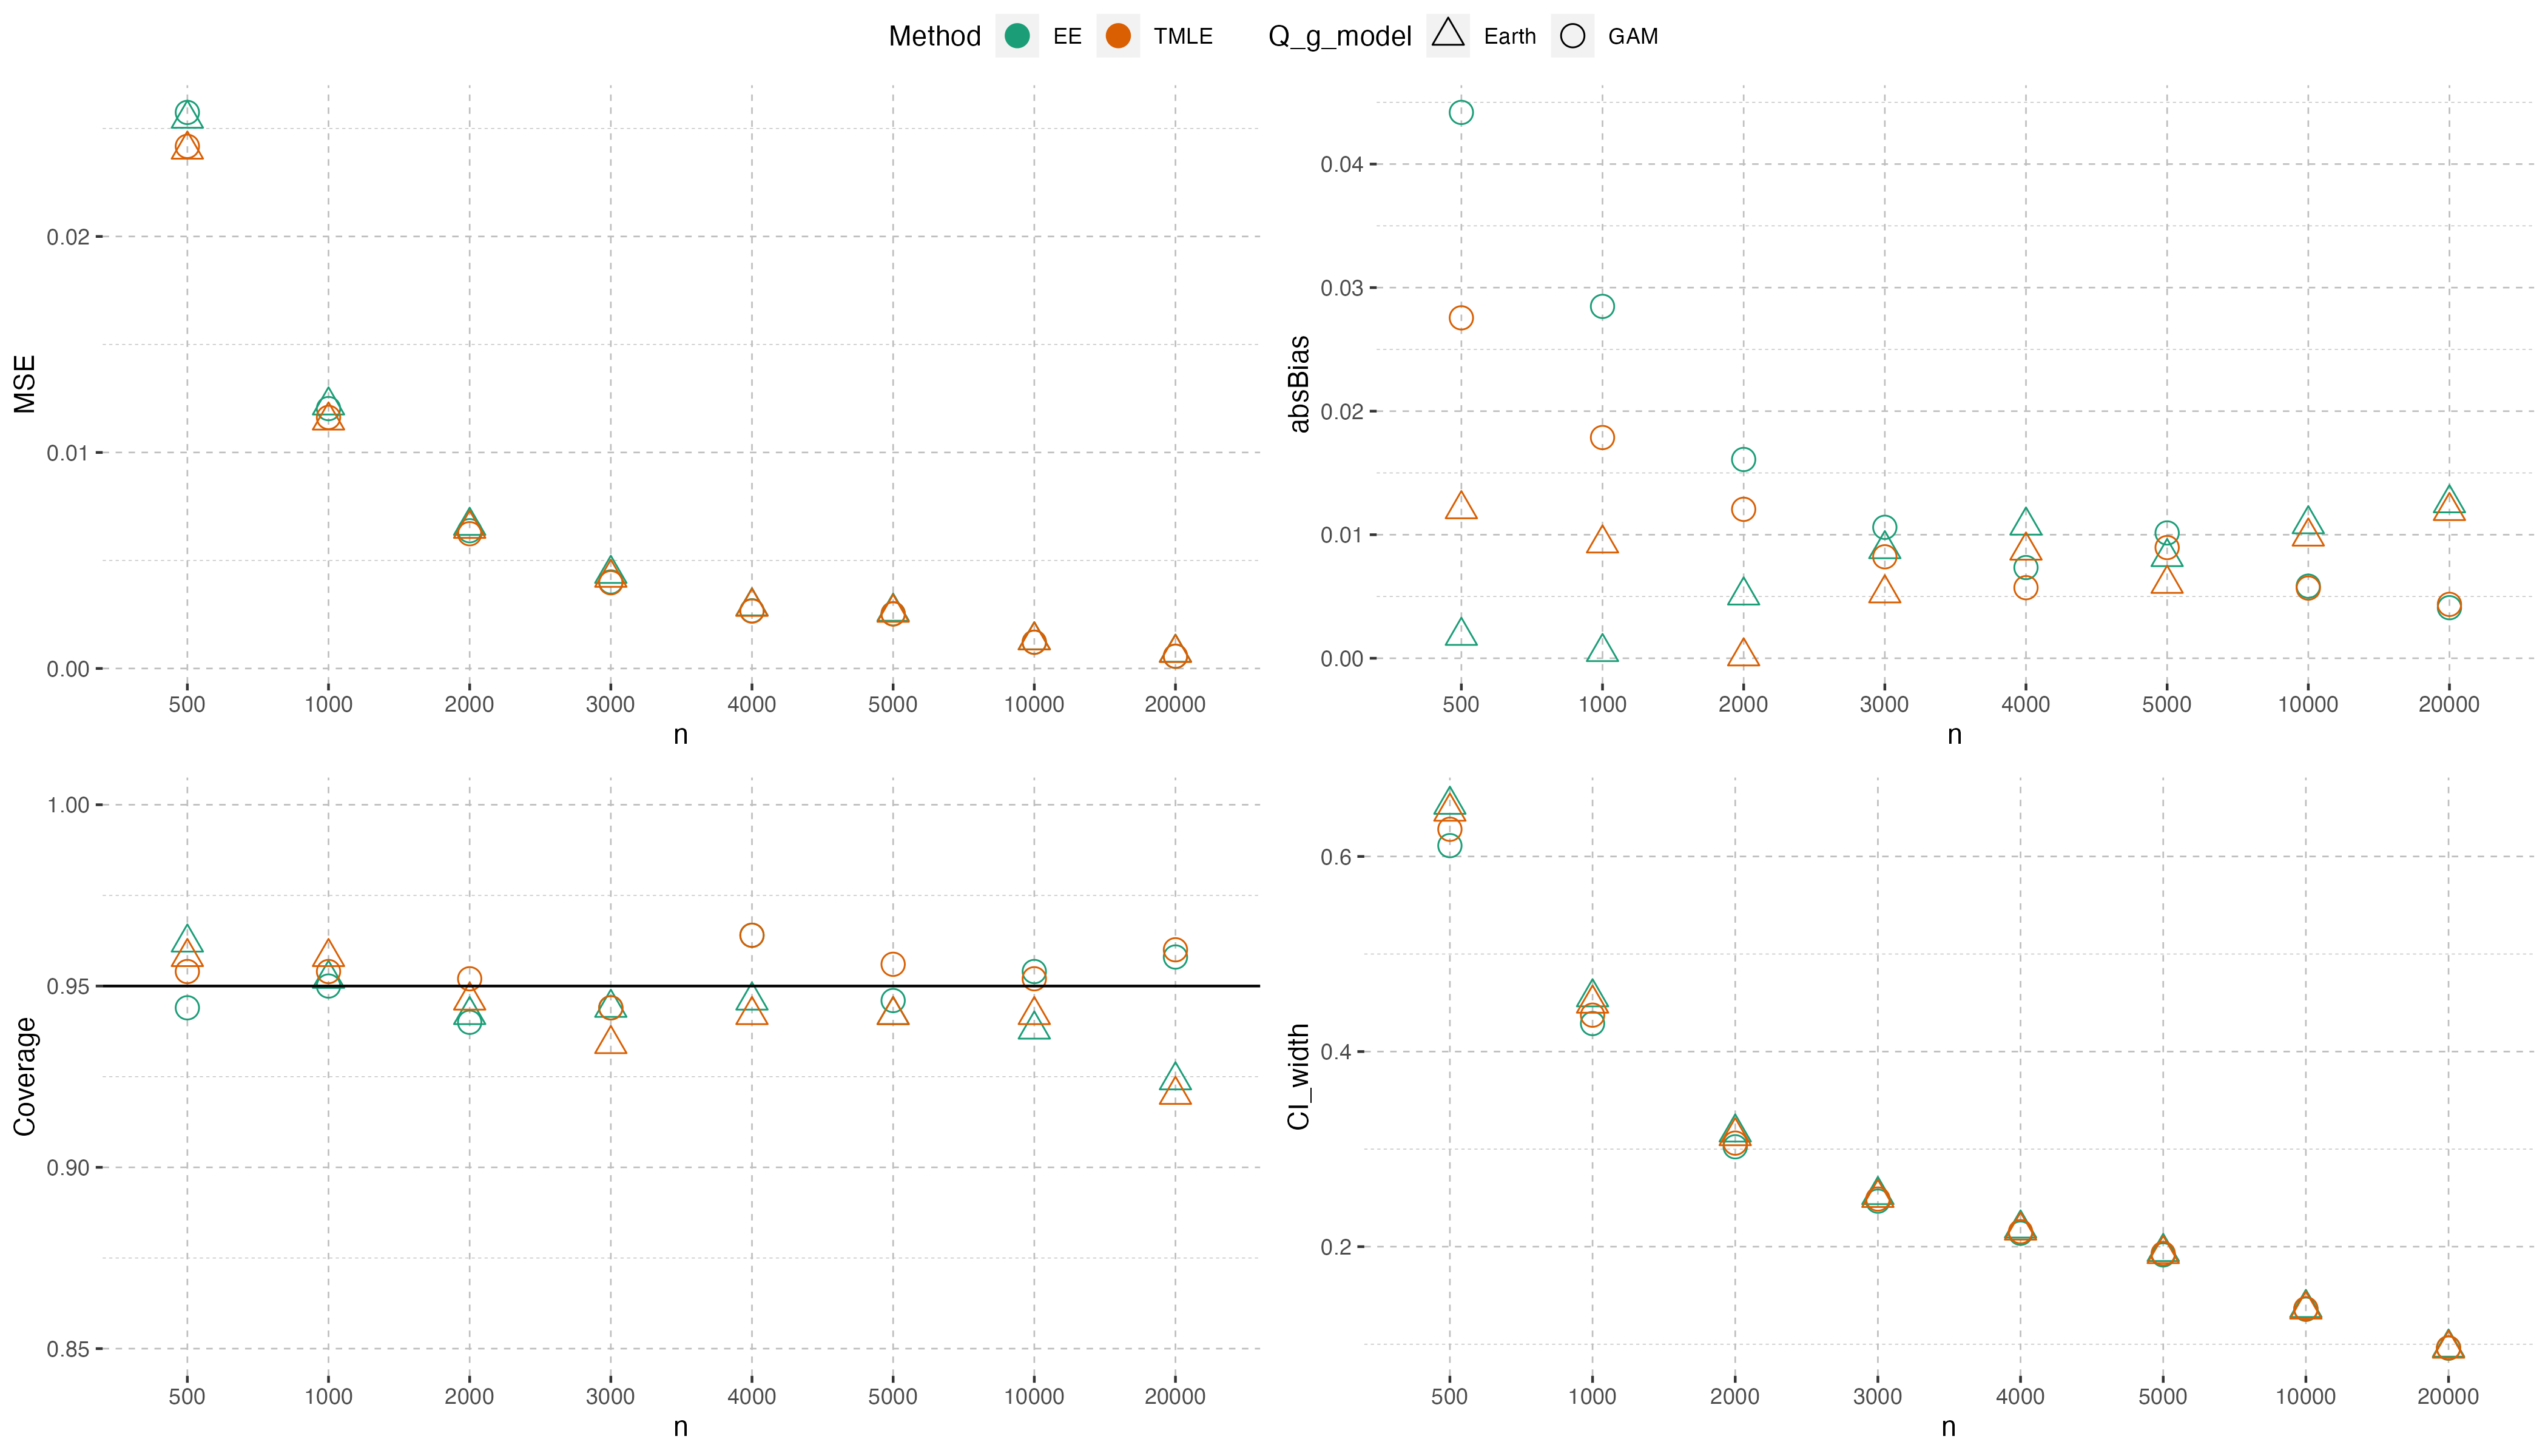
\includegraphics[width=1\linewidth]{plot_dots_t_nocv_v} 

}

\caption{Main performance metrics (T-learner, no CV)}\label{fig:unnamed-chunk-15}
\end{figure}

\begin{figure}[H]

{\centering 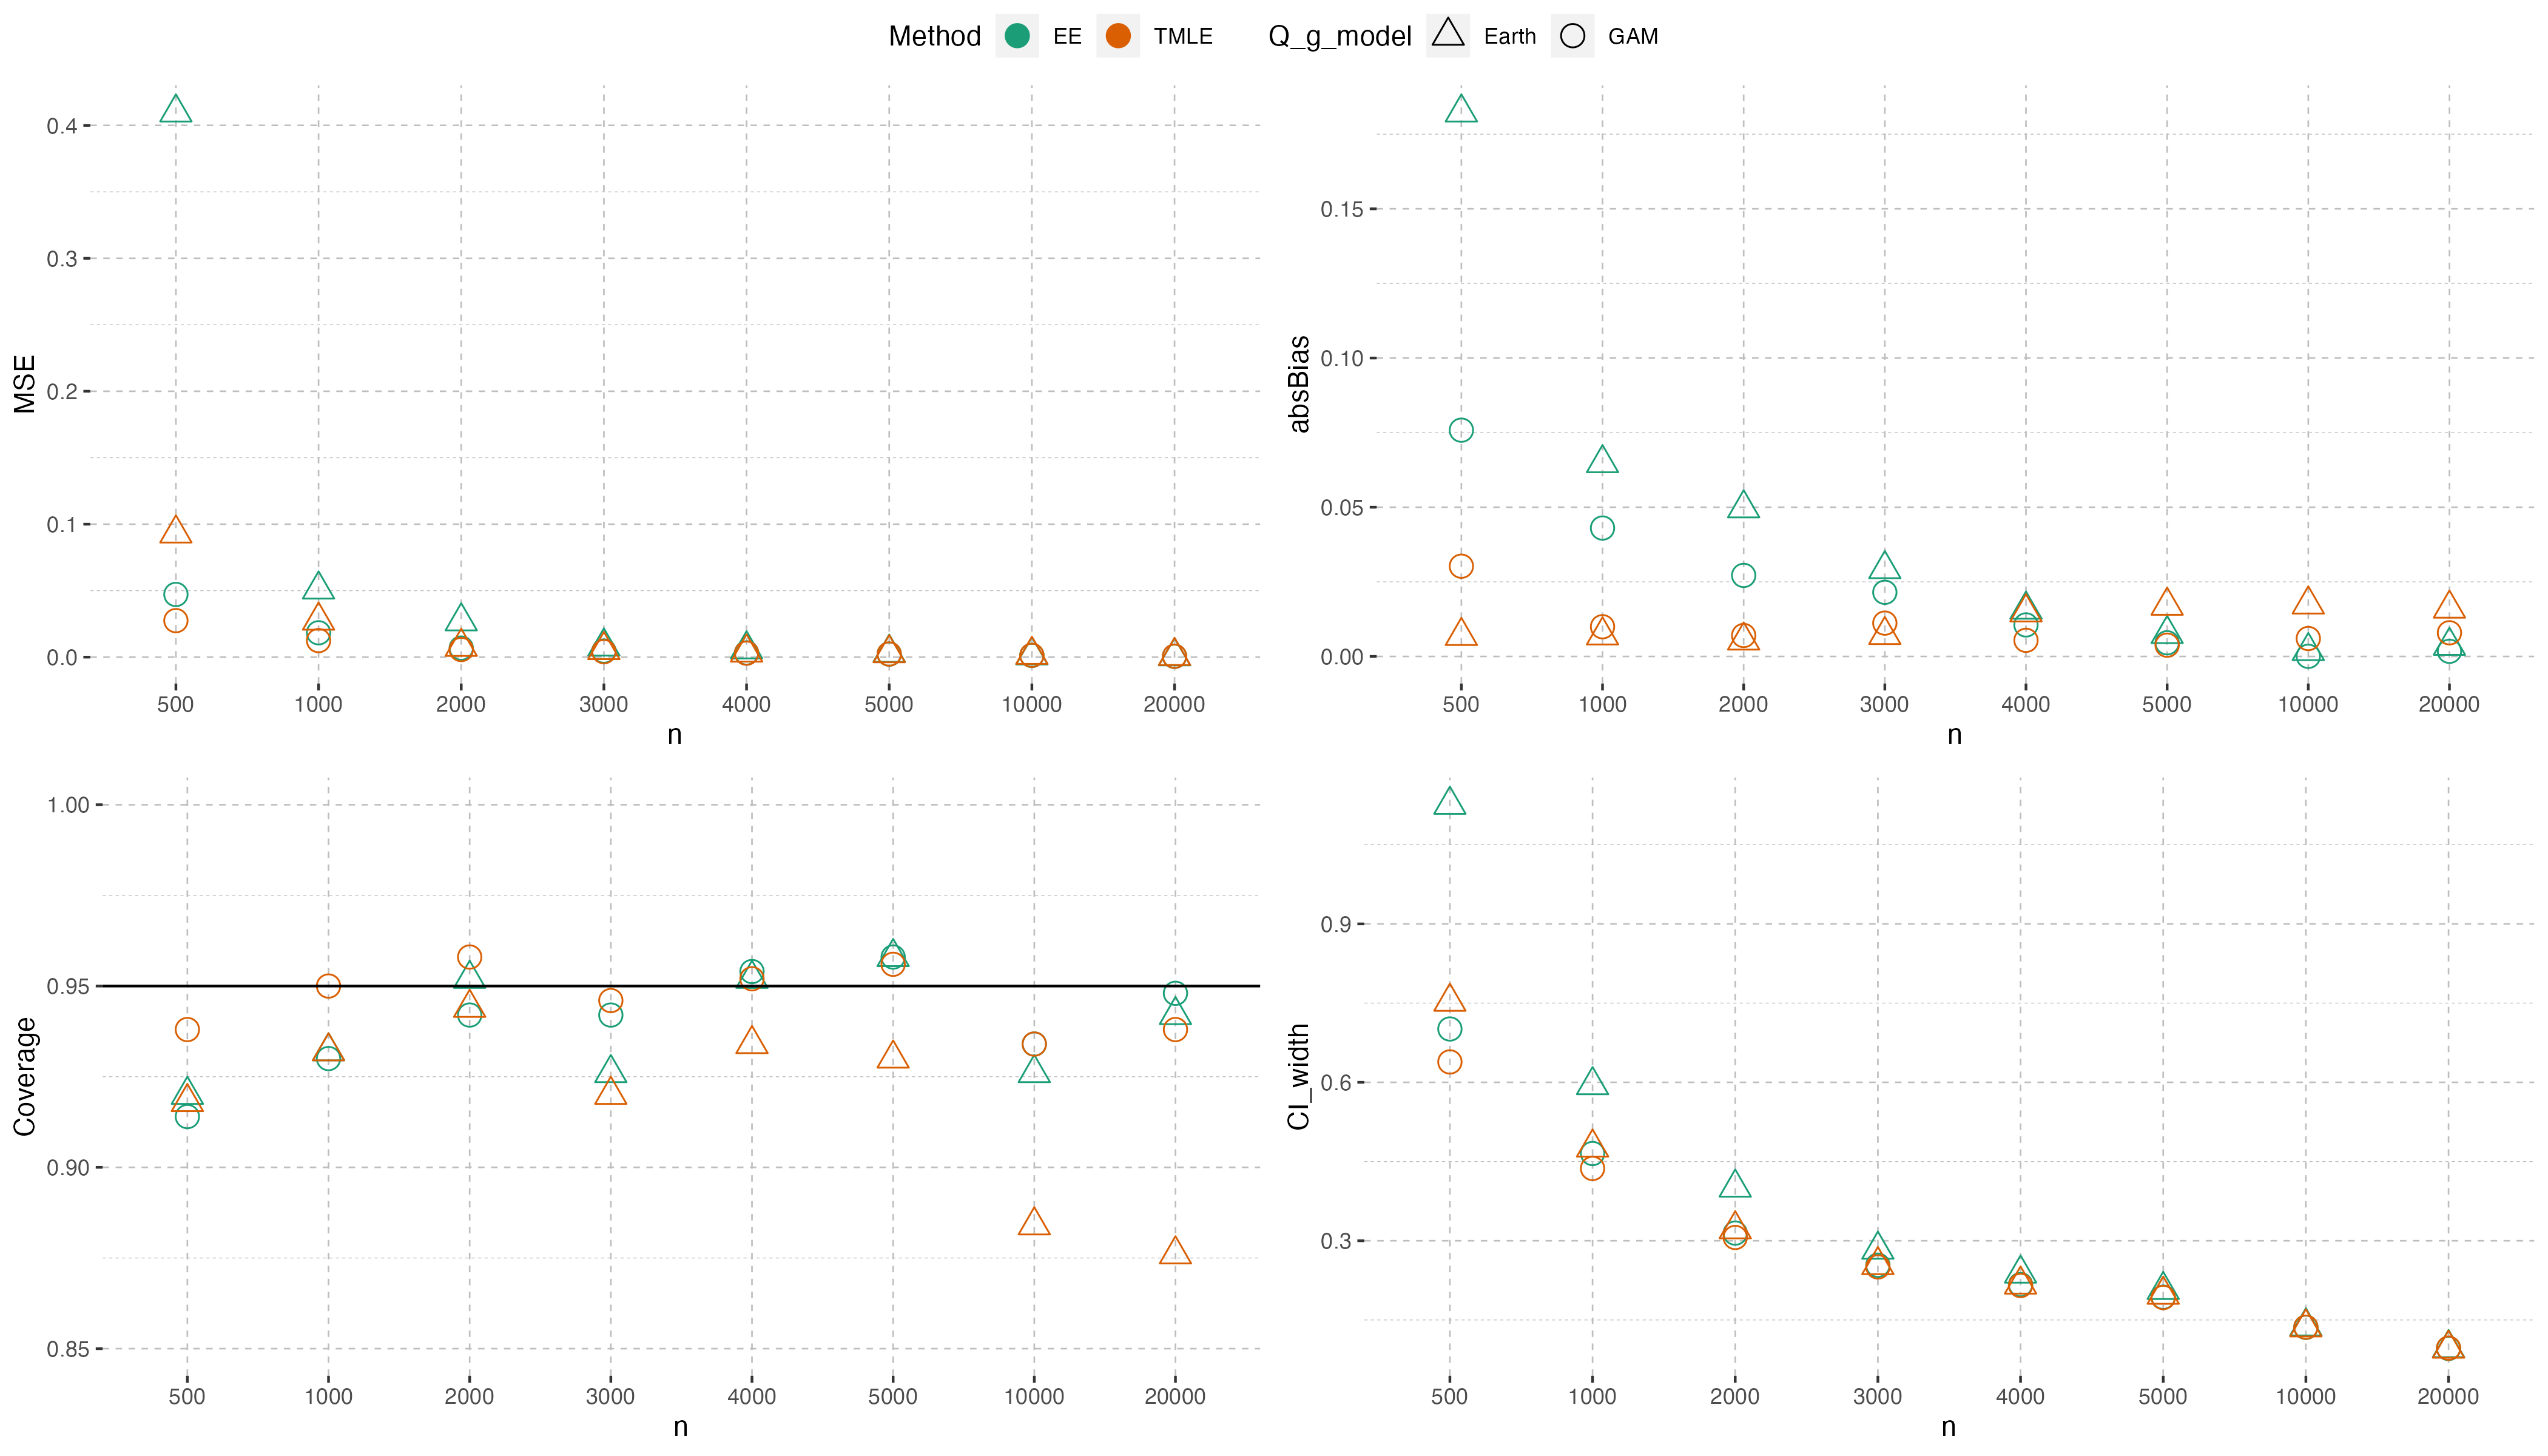
\includegraphics[width=1\linewidth]{plot_dots_dr_nocv_v} 

}

\caption{Main performance metrics (DR-learner, no CV)}\label{fig:unnamed-chunk-16}
\end{figure}

\begin{figure}[H]

{\centering 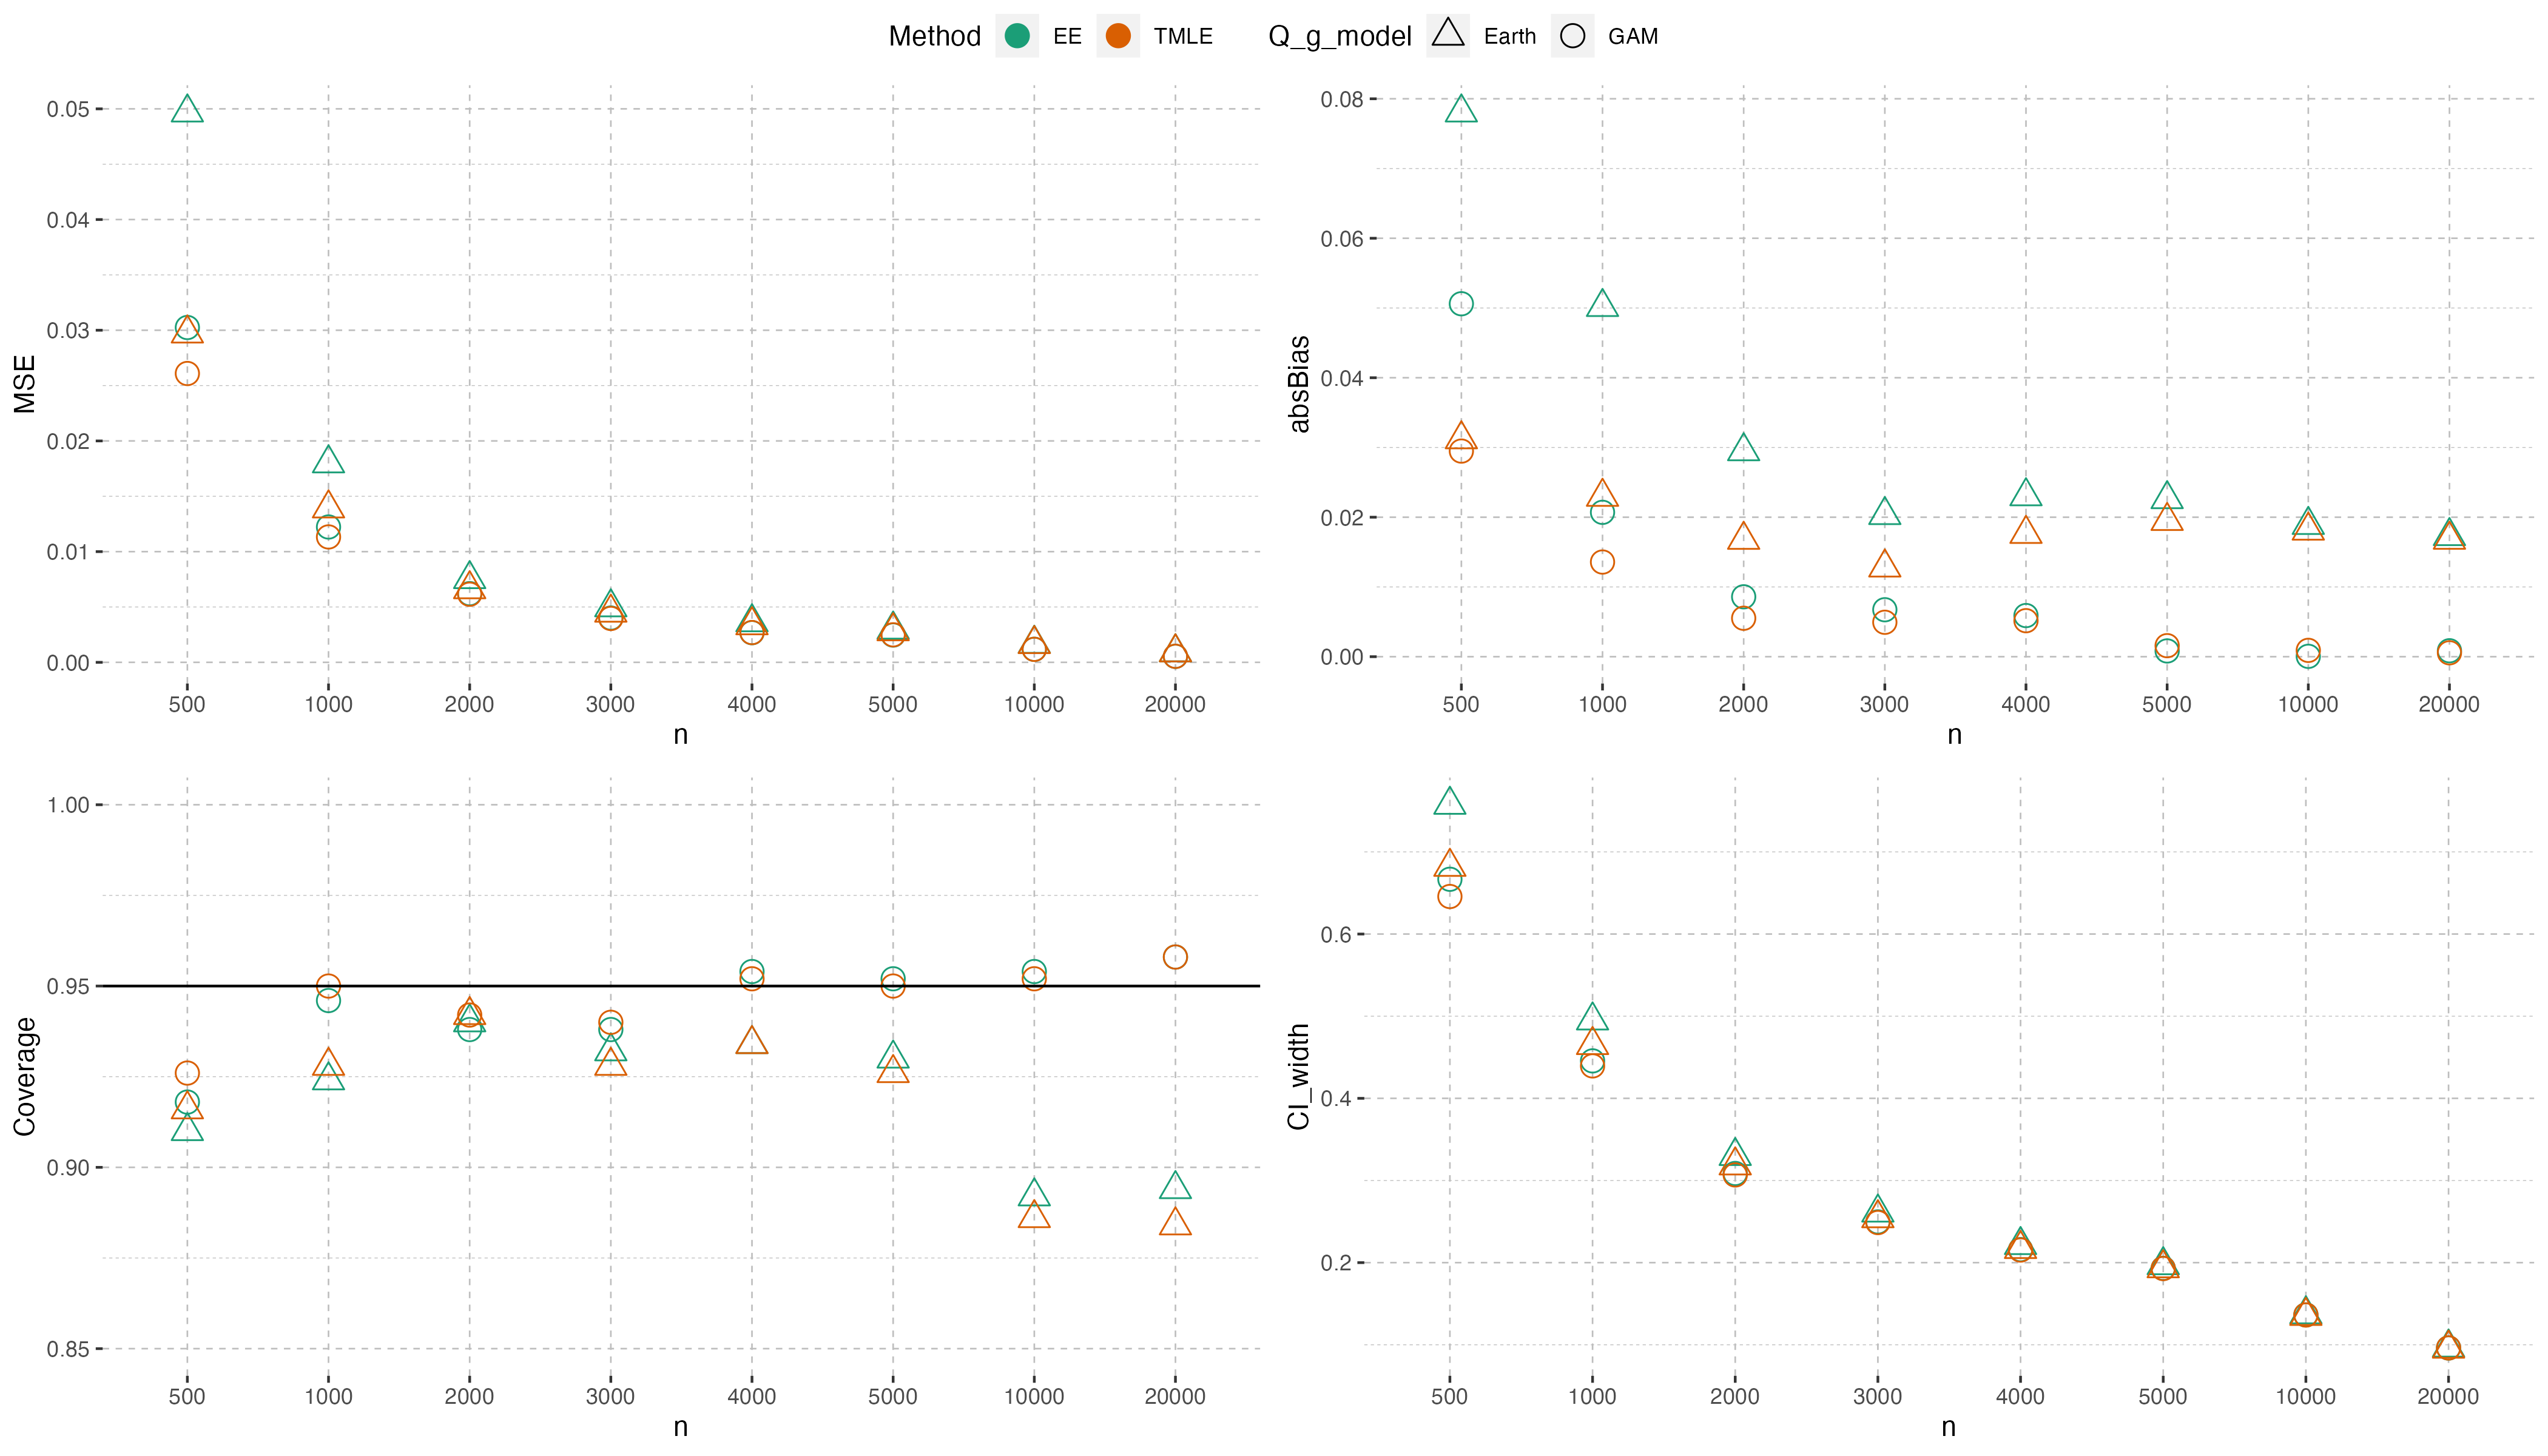
\includegraphics[width=1\linewidth]{plot_dots_t_cv_v} 

}

\caption{Main performance metrics (T-learner, CV)}\label{fig:unnamed-chunk-17}
\end{figure}

\begin{figure}[H]

{\centering 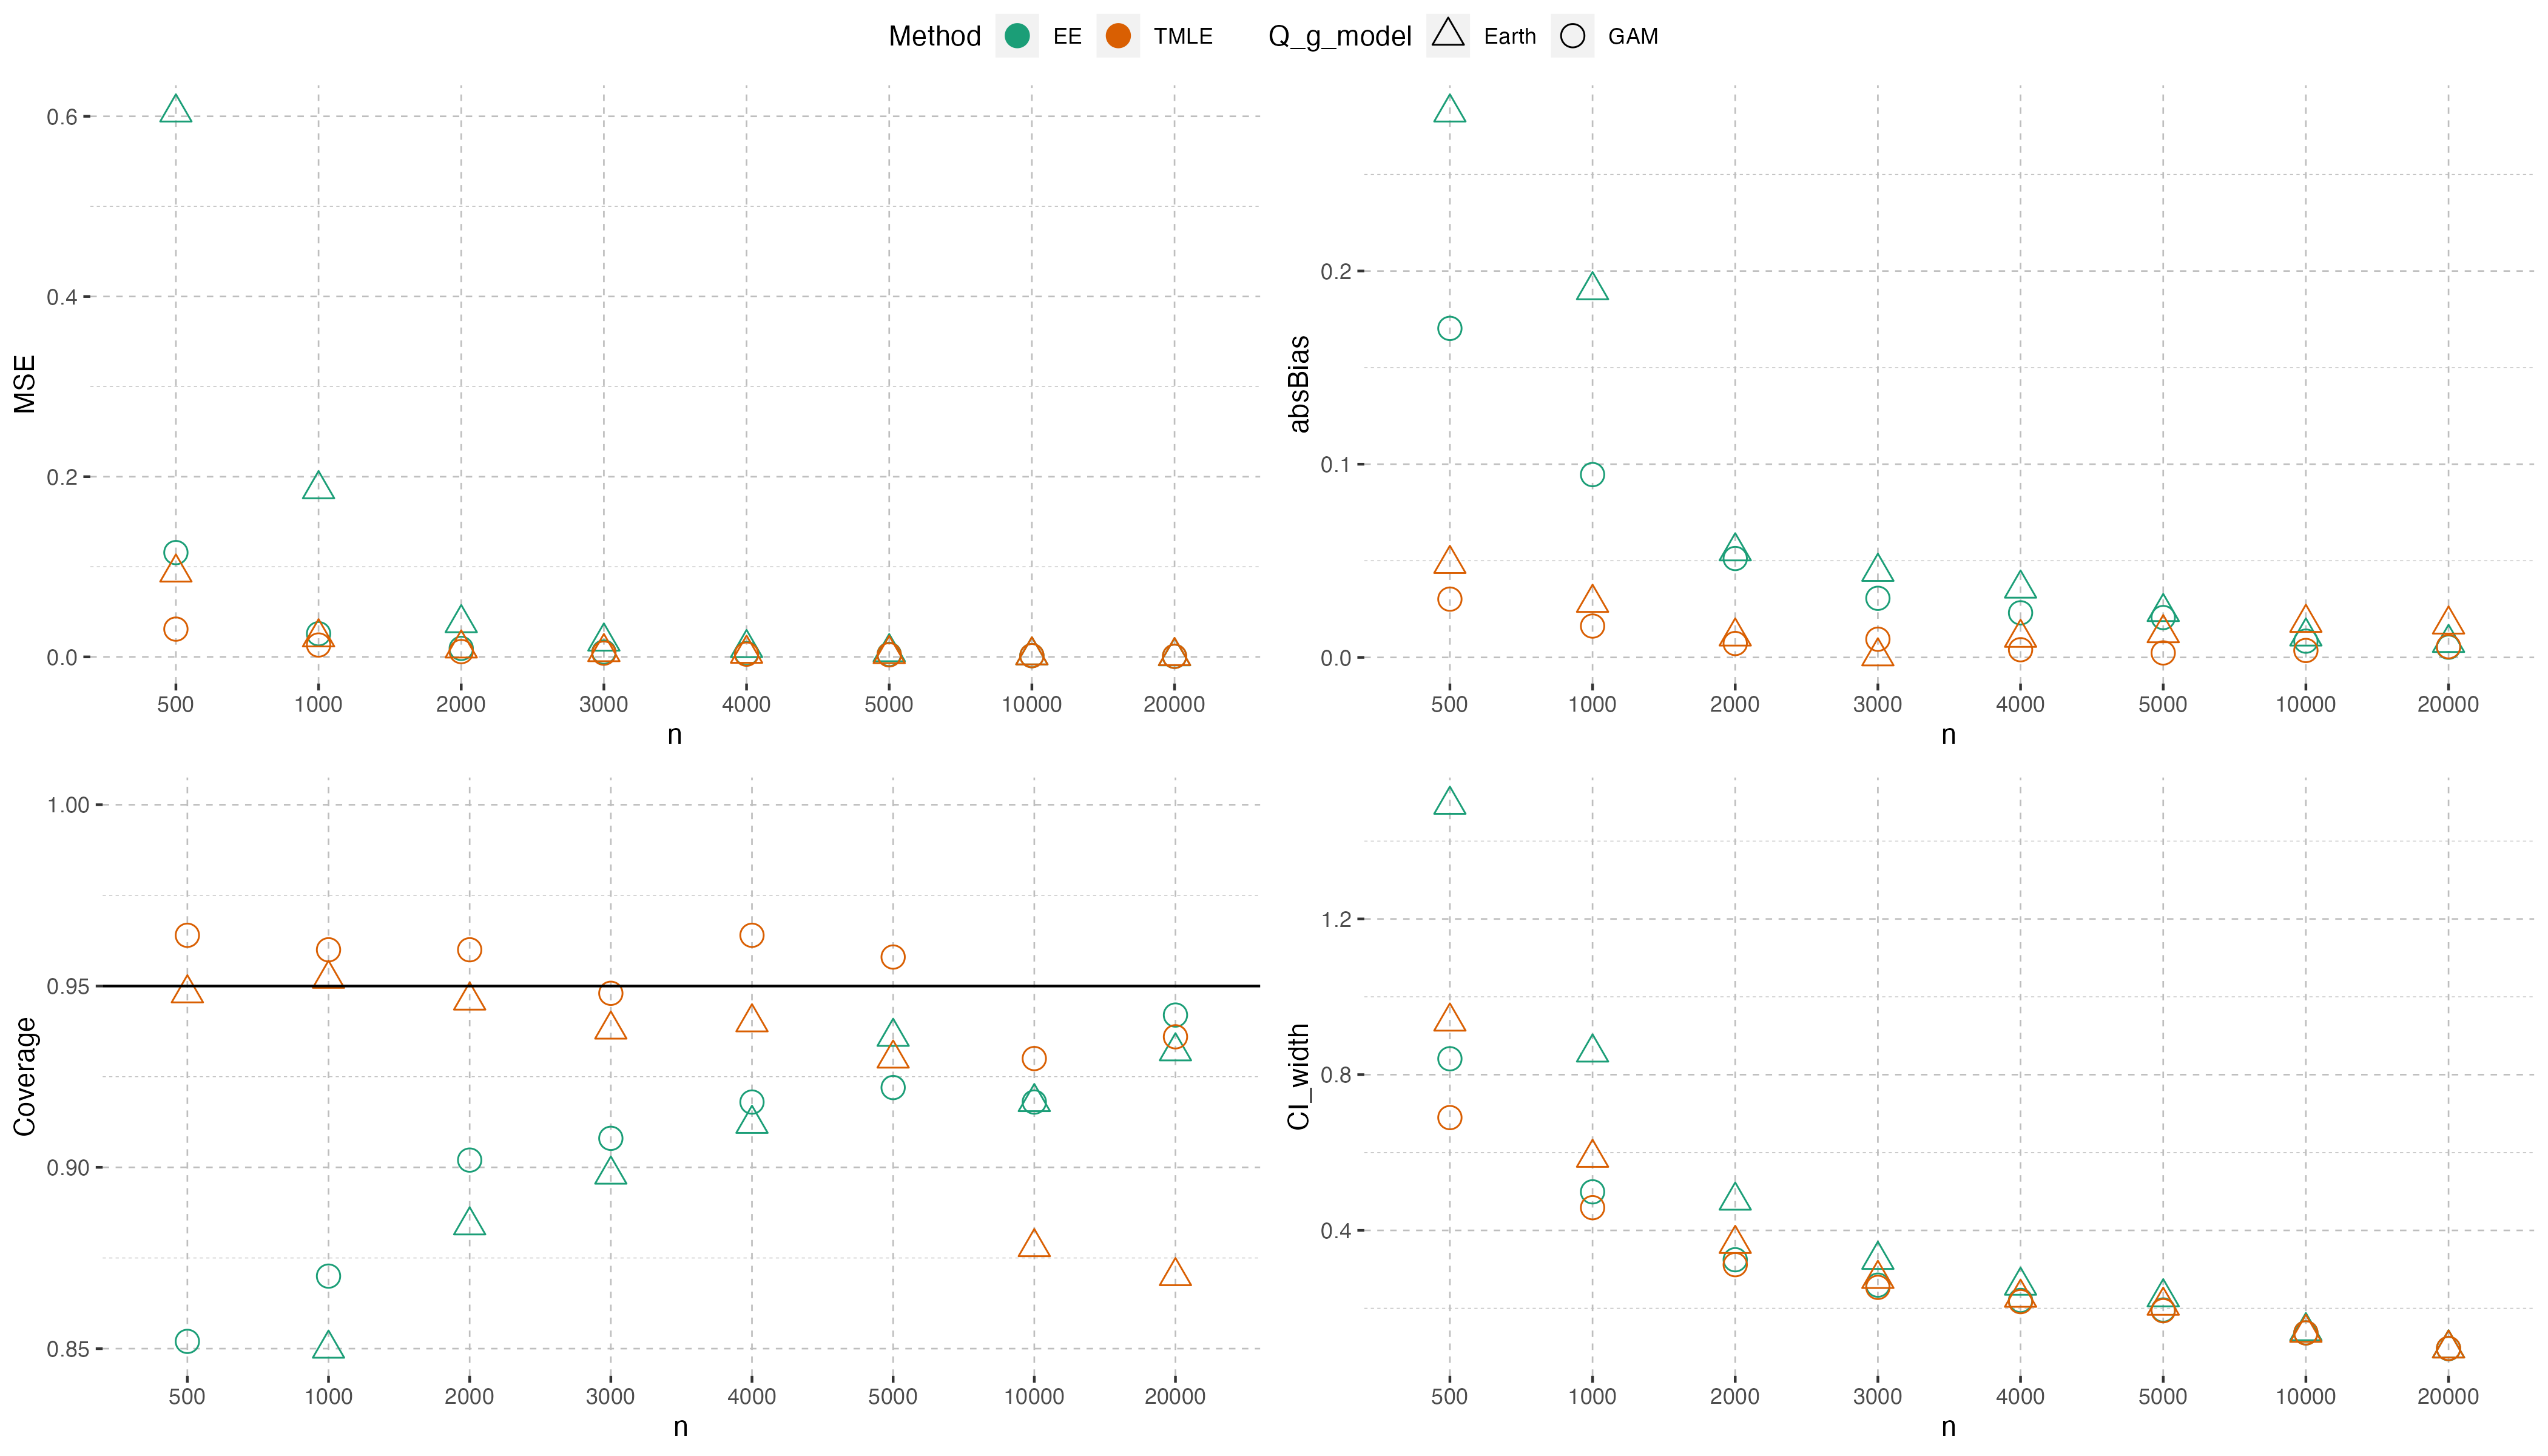
\includegraphics[width=1\linewidth]{plot_dots_dr_cv_v} 

}

\caption{Main performance metrics (DR-learner, CV)}\label{fig:unnamed-chunk-18}
\end{figure}

\begin{figure}[H]

{\centering 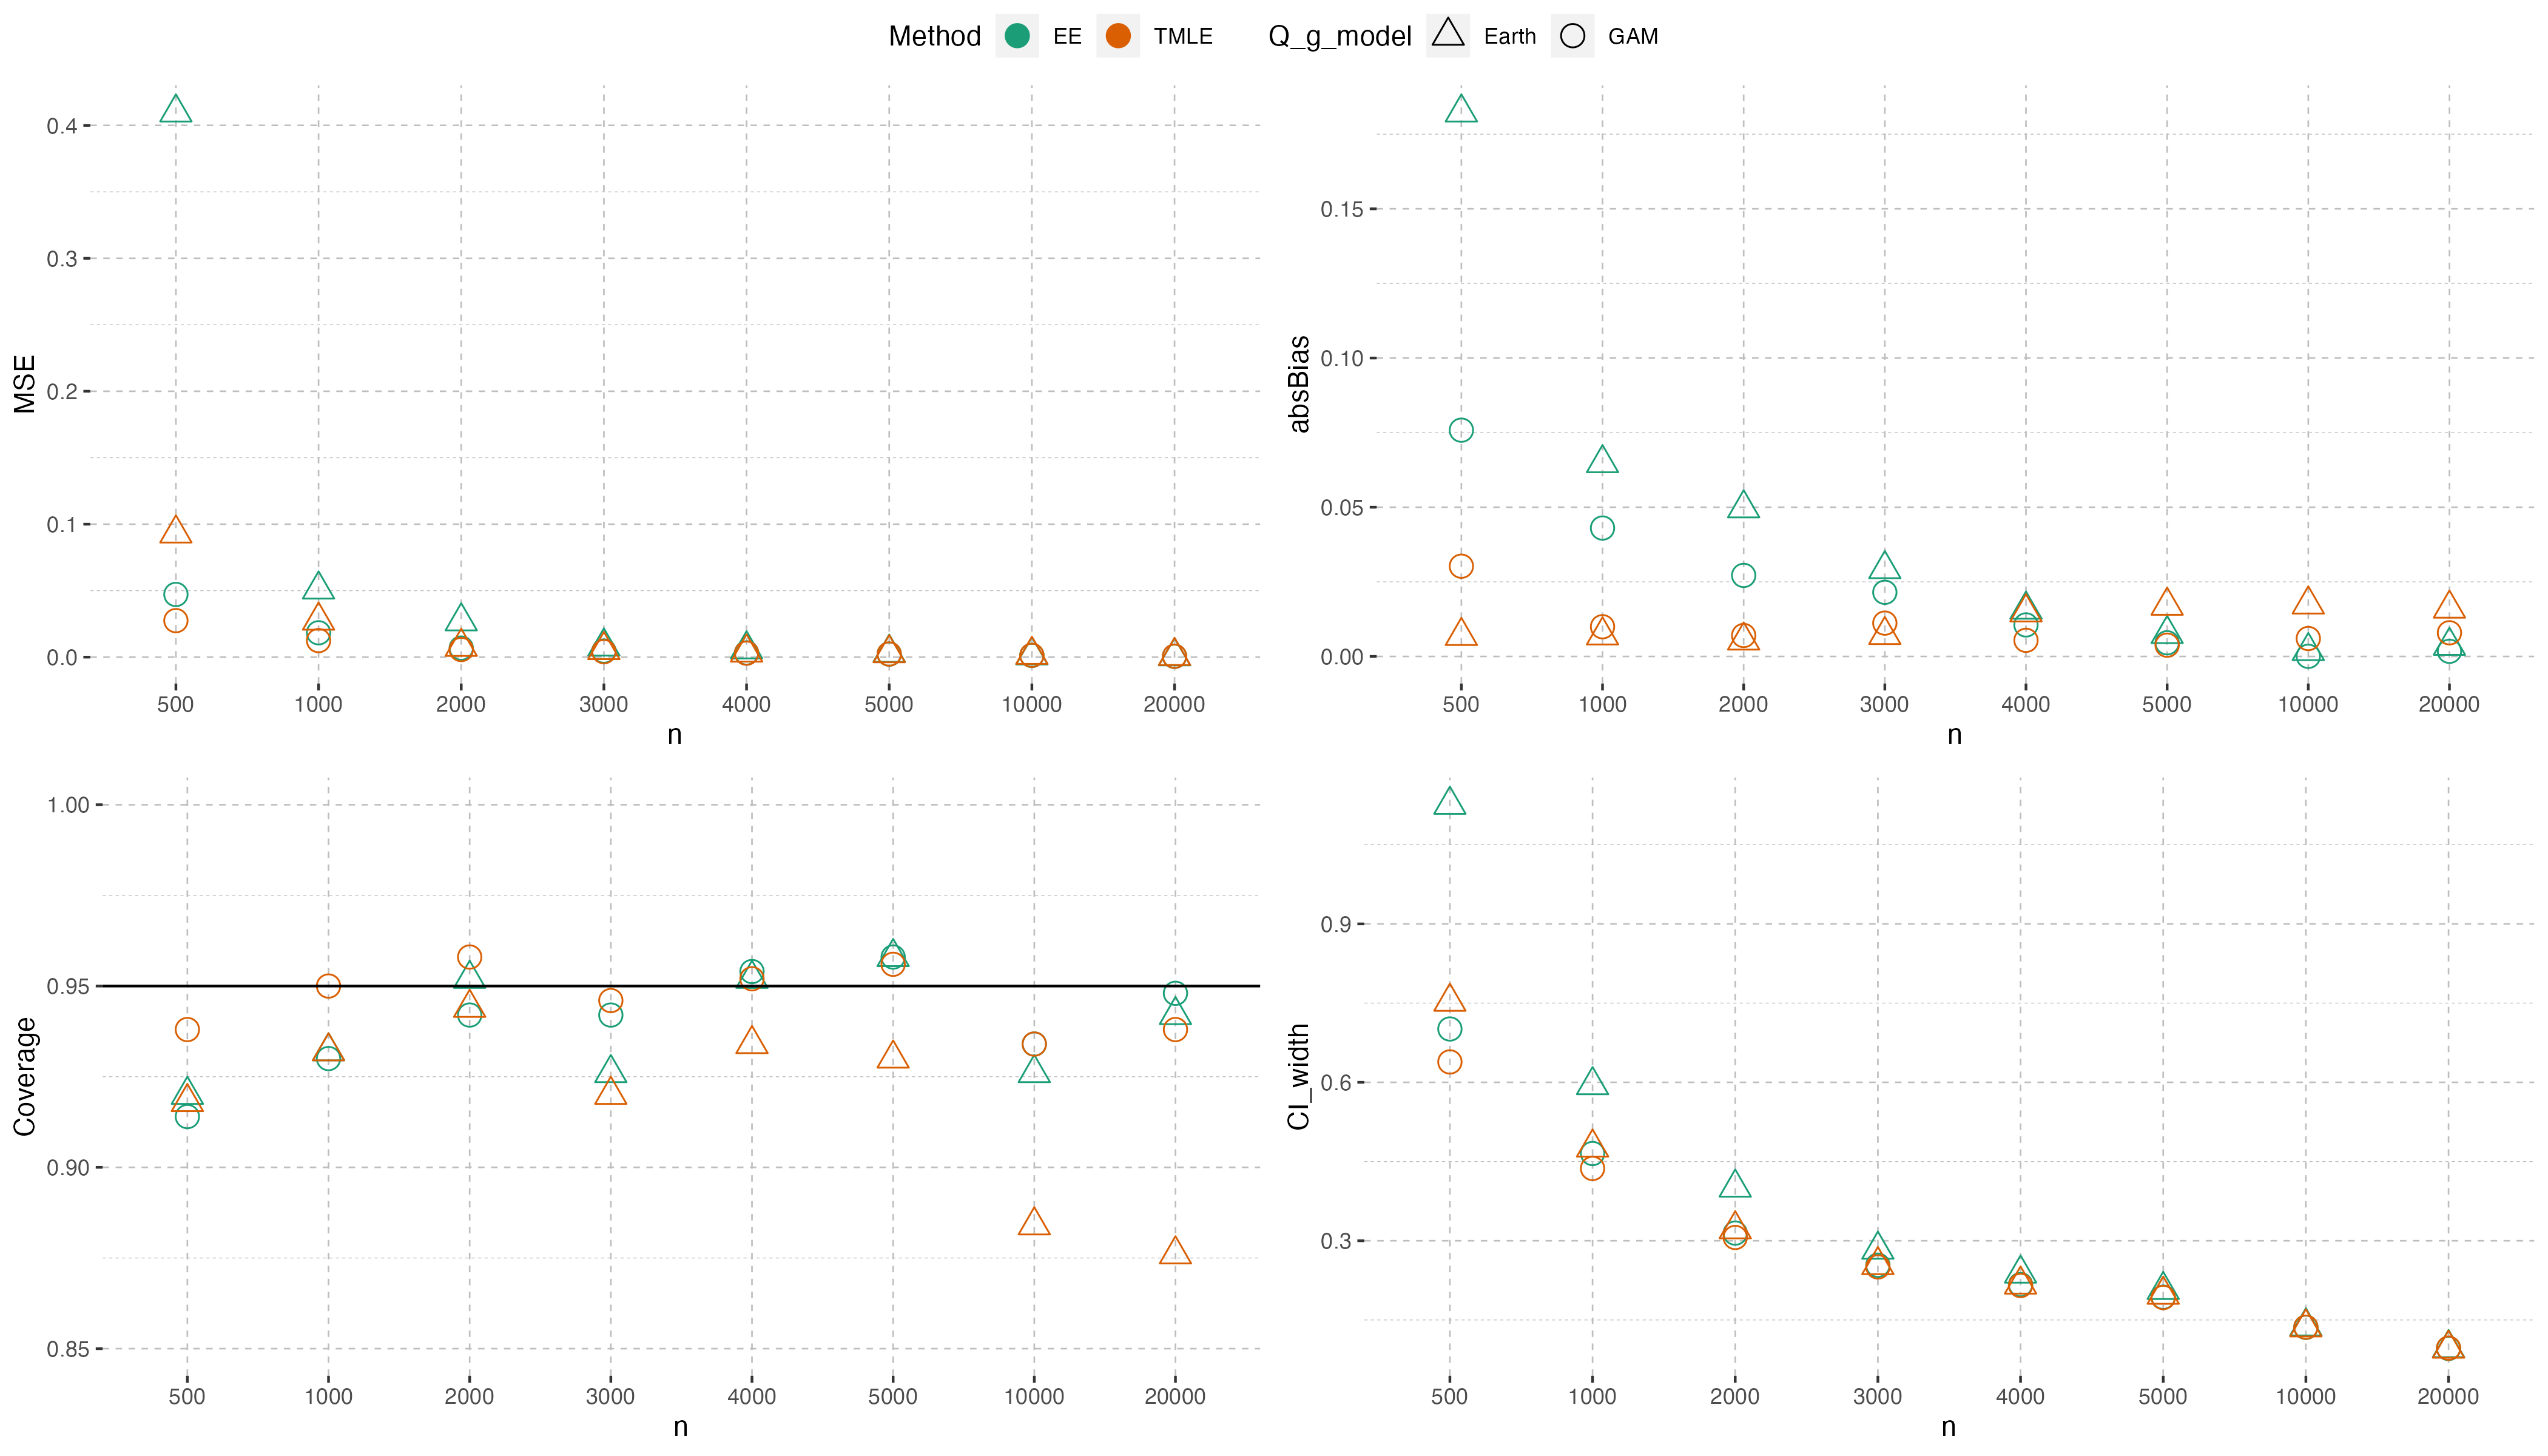
\includegraphics[width=1\linewidth]{plot_dots_dr_nocv_v} 

}

\caption{Main performance metrics (DR-learner, no CV)}\label{fig:unnamed-chunk-19}
\end{figure}

\begin{figure}[H]

{\centering 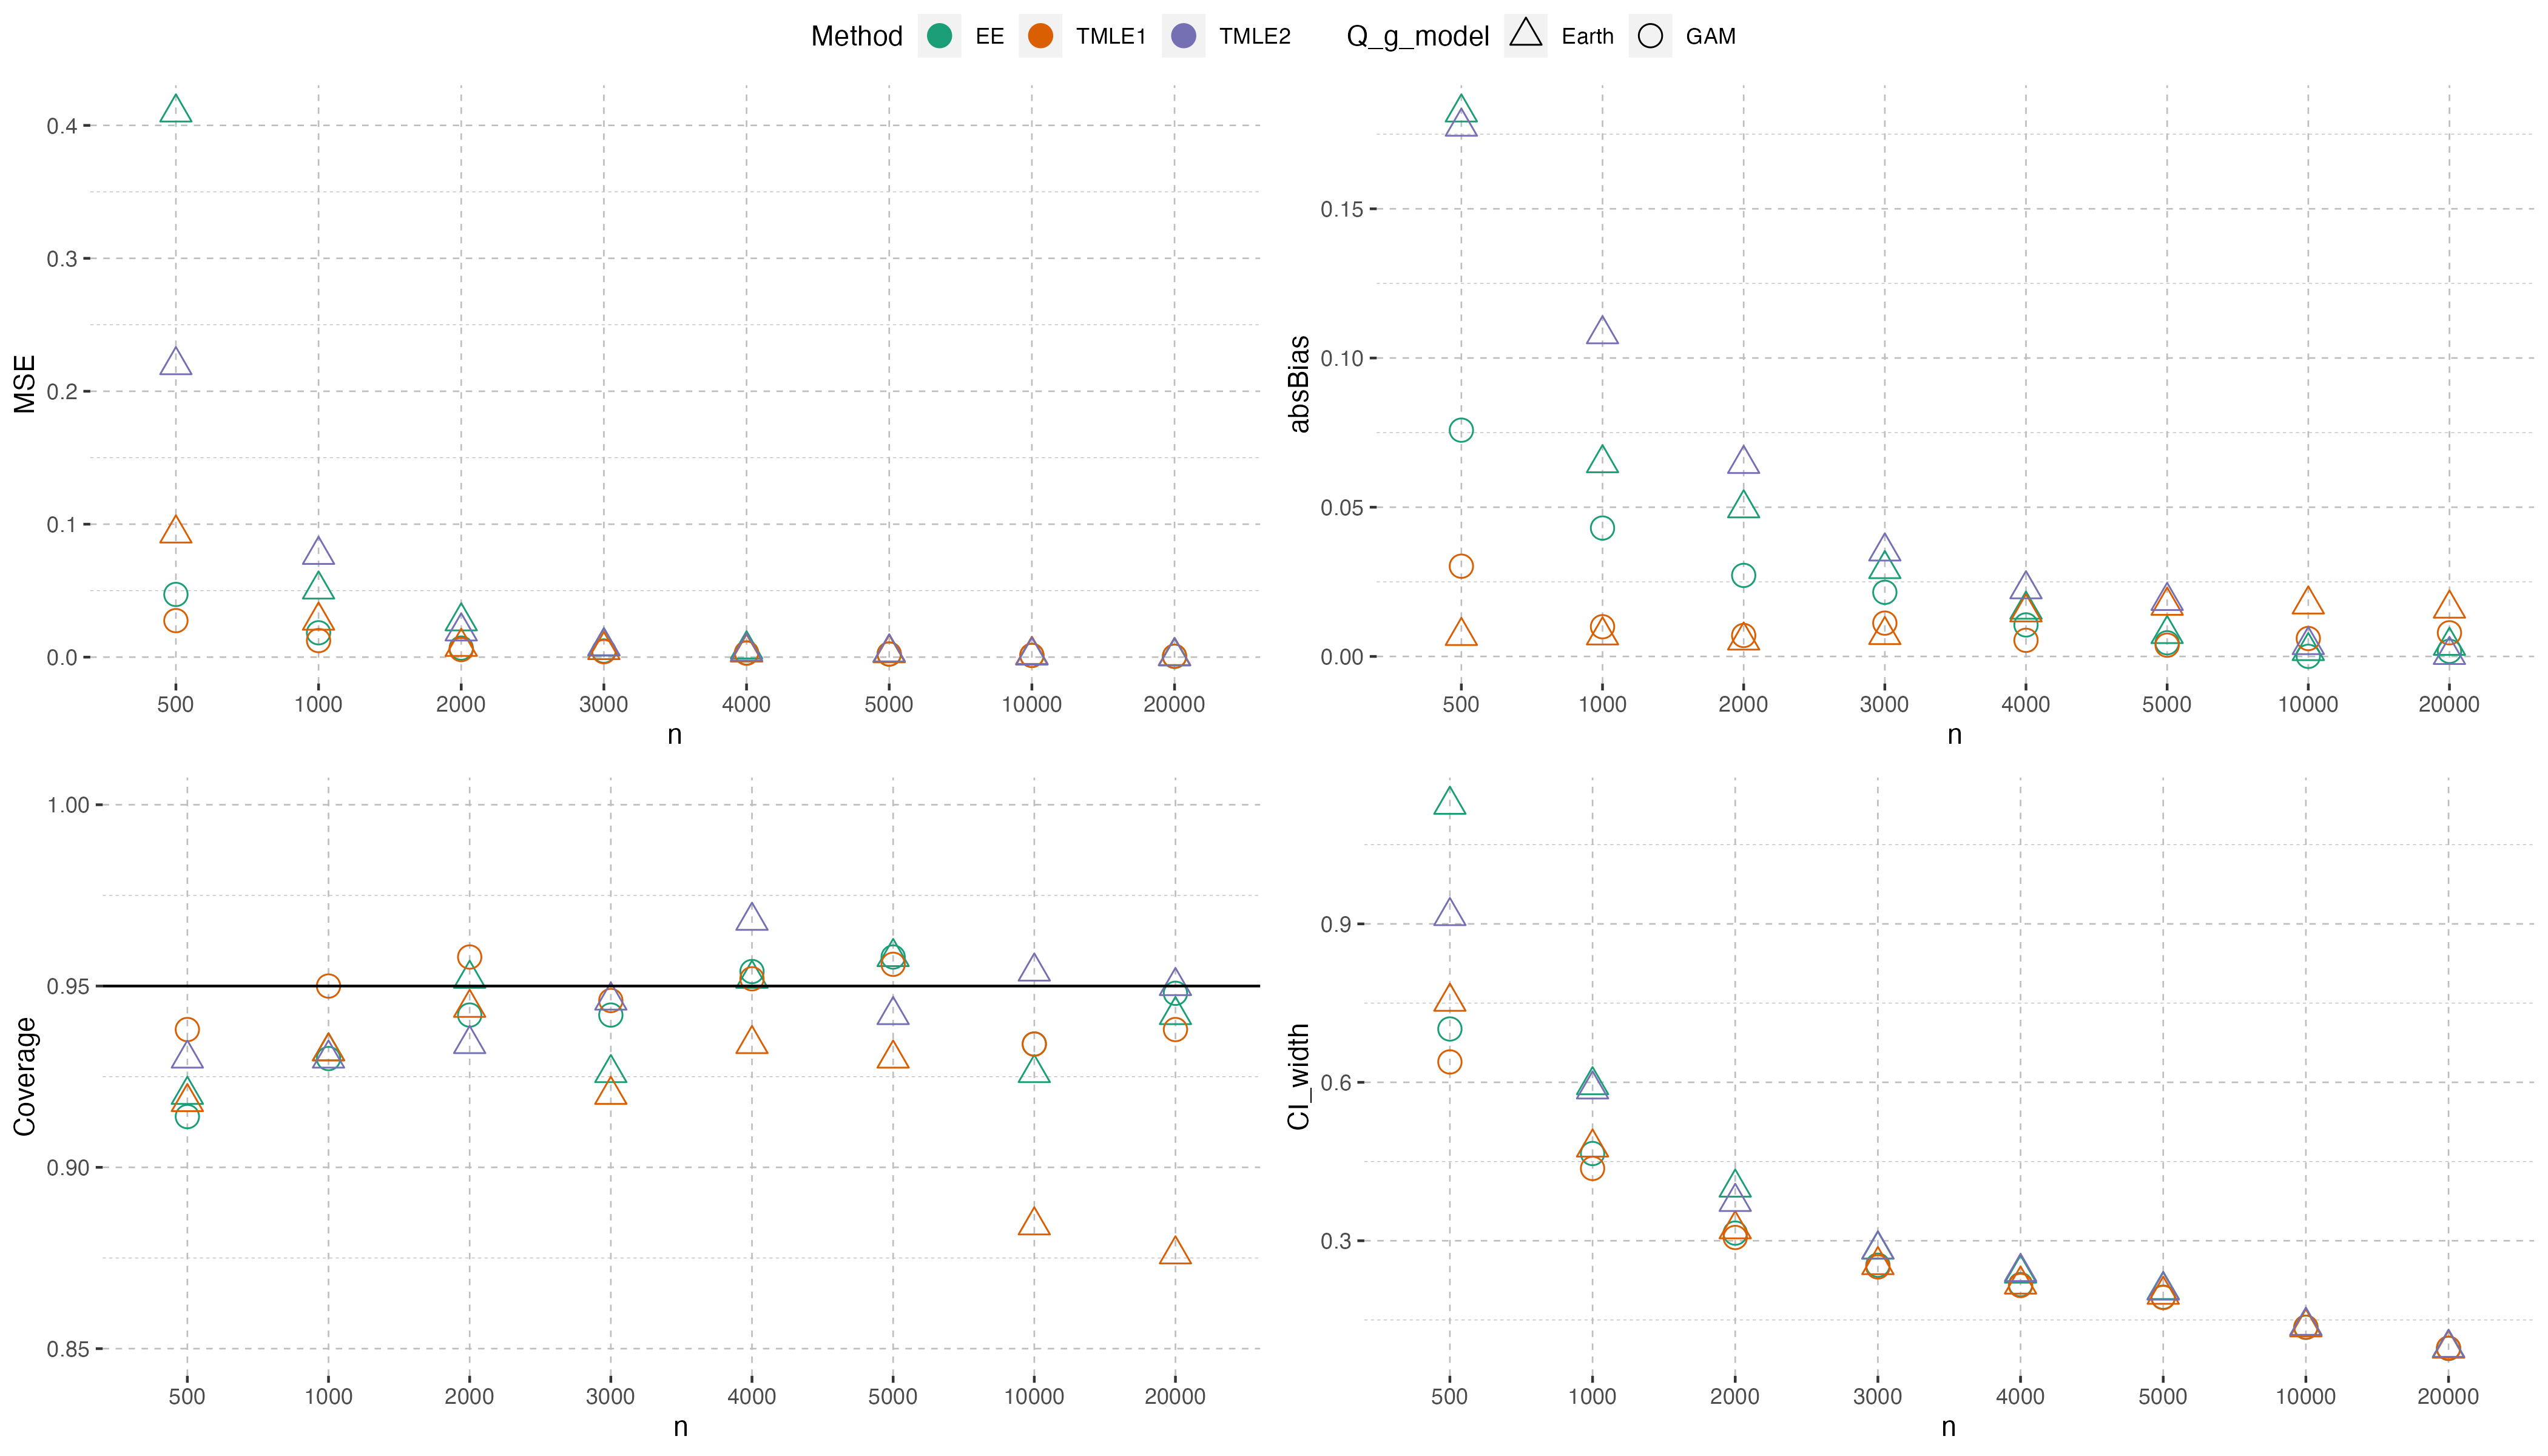
\includegraphics[width=1\linewidth]{plot_dots_dr_nocv_new_v} 

}

\caption{Main performance metrics (DR-learner, no CV)}\label{fig:unnamed-chunk-20}
\end{figure}

\begin{table}

\caption{\label{tab:unnamed-chunk-21}Performance of TMLE (with DR CATE update) and EE for Theta (earth est Q and g, DR-learner, no CV)}
\centering
\resizebox{\linewidth}{!}{
\begin{tabular}[t]{rlrrrrrrr}
\toprule
n & Method & True\_Theta & Variance & Bias & MSE & Coverage & Coverage\_or & CI\_width\\
\midrule
 & TMLE & 0.686 & 0.1881 & 0.1775 & 0.2196 & 0.930 & 0.954 & 0.9148\\

\multirow{-2}{*}{\raggedleft\arraybackslash 500} & EE & 0.686 & 0.1354 & 0.1185 & 0.1495 & 0.930 & 0.952 & 1.0280\\
\cmidrule{1-9}
 & TMLE & 0.686 & 0.0653 & 0.1080 & 0.0769 & 0.930 & 0.964 & 0.5865\\

\multirow{-2}{*}{\raggedleft\arraybackslash 1000} & EE & 0.686 & 0.0394 & 0.0628 & 0.0434 & 0.938 & 0.962 & 0.6009\\
\cmidrule{1-9}
 & TMLE & 0.686 & 0.0152 & 0.0645 & 0.0194 & 0.934 & 0.948 & 0.3735\\

\multirow{-2}{*}{\raggedleft\arraybackslash 2000} & EE & 0.686 & 0.0153 & 0.0465 & 0.0174 & 0.928 & 0.966 & 0.3931\\
\cmidrule{1-9}
 & TMLE & 0.686 & 0.0070 & 0.0352 & 0.0083 & 0.946 & 0.962 & 0.2836\\

\multirow{-2}{*}{\raggedleft\arraybackslash 3000} & EE & 0.686 & 0.0078 & 0.0259 & 0.0084 & 0.952 & 0.980 & 0.2897\\
\cmidrule{1-9}
 & TMLE & 0.686 & 0.0038 & 0.0225 & 0.0043 & 0.968 & 0.954 & 0.2409\\

\multirow{-2}{*}{\raggedleft\arraybackslash 4000} & EE & 0.686 & 0.0039 & 0.0146 & 0.0042 & 0.968 & 0.960 & 0.2438\\
\cmidrule{1-9}
 & TMLE & 0.686 & 0.0033 & 0.0186 & 0.0036 & 0.942 & 0.942 & 0.2057\\

\multirow{-2}{*}{\raggedleft\arraybackslash 5000} & EE & 0.686 & 0.0033 & 0.0127 & 0.0035 & 0.950 & 0.960 & 0.2083\\
\cmidrule{1-9}
 & TMLE & 0.686 & 0.0012 & 0.0038 & 0.0012 & 0.954 & 0.950 & 0.1390\\

\multirow{-2}{*}{\raggedleft\arraybackslash 10000} & EE & 0.686 & 0.0012 & 0.0009 & 0.0012 & 0.954 & 0.948 & 0.1392\\
\cmidrule{1-9}
 & TMLE & 0.686 & 0.0006 & 0.0005 & 0.0006 & 0.950 & 0.948 & 0.0972\\

\multirow{-2}{*}{\raggedleft\arraybackslash 20000} & EE & 0.686 & 0.0006 & -0.0021 & 0.0006 & 0.948 & 0.950 & 0.0971\\
\bottomrule
\end{tabular}}
\end{table}

\end{document}
